\section*{Problema 7}

\textbf{Durante los juegos olimpicos de Salt Lake City surgió en un periódico la discusión si en las pruebas de 1500m de patinaje, la persona en el carril exterior no tendria ventaja sobre el carril interior. Se organizaron 24 pruebas (una se canceló por una caida). Abajo los tiempos. Aplica una(s) pruebas de estadistica relevante para contestar esta pregunta.}

En la tabla \ref{table:problema07} se encuentran las medidas de tendencia central y despersión de los datos contenidos en el archivo \file{data.csv}. Se observa que estas medidas son semejantes entre los dos conjuntos, en donde existe una mayor diferencia es en la varianza.

\begin{table}[H]
	\centering
	\begin{tabular}{cccc} \hline
		\textbf{Linea} & \textbf{Mediana (s)} & \textbf{Promedio (s)} & \textbf{Varianza (s\textsuperscript{2})} \\ \hline
		Interna        & 107.9                & 108.2                 & 2.9653                                   \\
		Externa        & 106.3                & 107.4                 & 6.3327                                   \\ \hline
	\end{tabular}
	\caption{Medidad de tendencia central y de dispersión de los datos.}
	\label{table:problema07}
\end{table}

Una primera aproximación para llegar a una conclusión es visualizar la distribución de datos por medio de boxplots (figura \ref{fig:problema07_boxplot}) y las frecuencias de los datos (figura \ref{fig:problema07_distribucion_datos}). Con esto podemos comprobar resultado obtenido en la tabla \ref{table:problema07}. Con esto podemos llegar a la aproximación que la hipótesis será rechazada. Esto debido a que los datos presentan distribuciones diferentes.

\begin{figure}[H]
	\centering
	\begin{subfigure}[b]{8cm}
		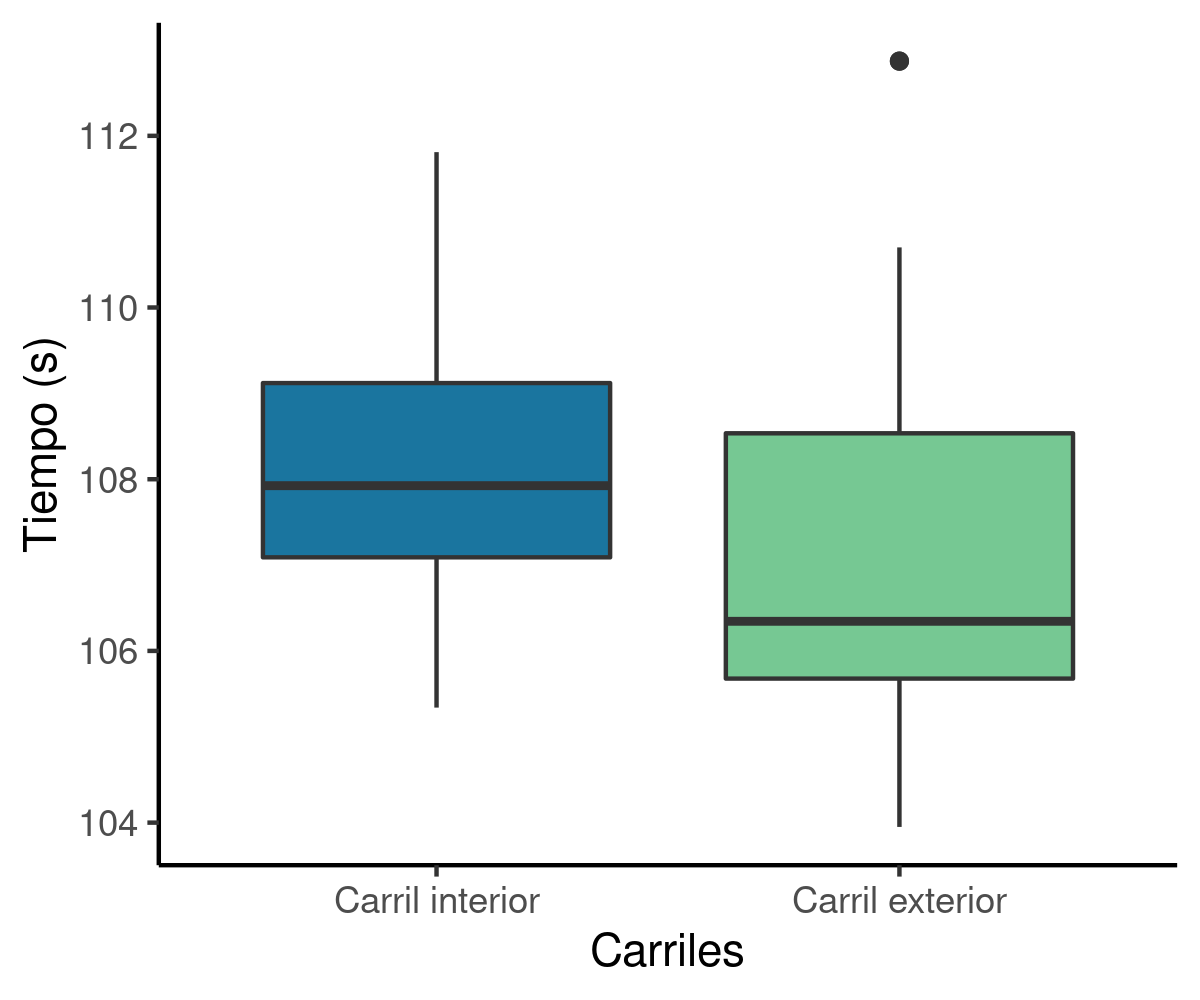
\includegraphics[width=8cm]{Graphics/problema07_boxplot.png}
		\caption{Boxplot de los datos del carril interior y exterior.}
		\label{fig:problema07_boxplot}
	\end{subfigure}
	\begin{subfigure}[b]{8cm}
		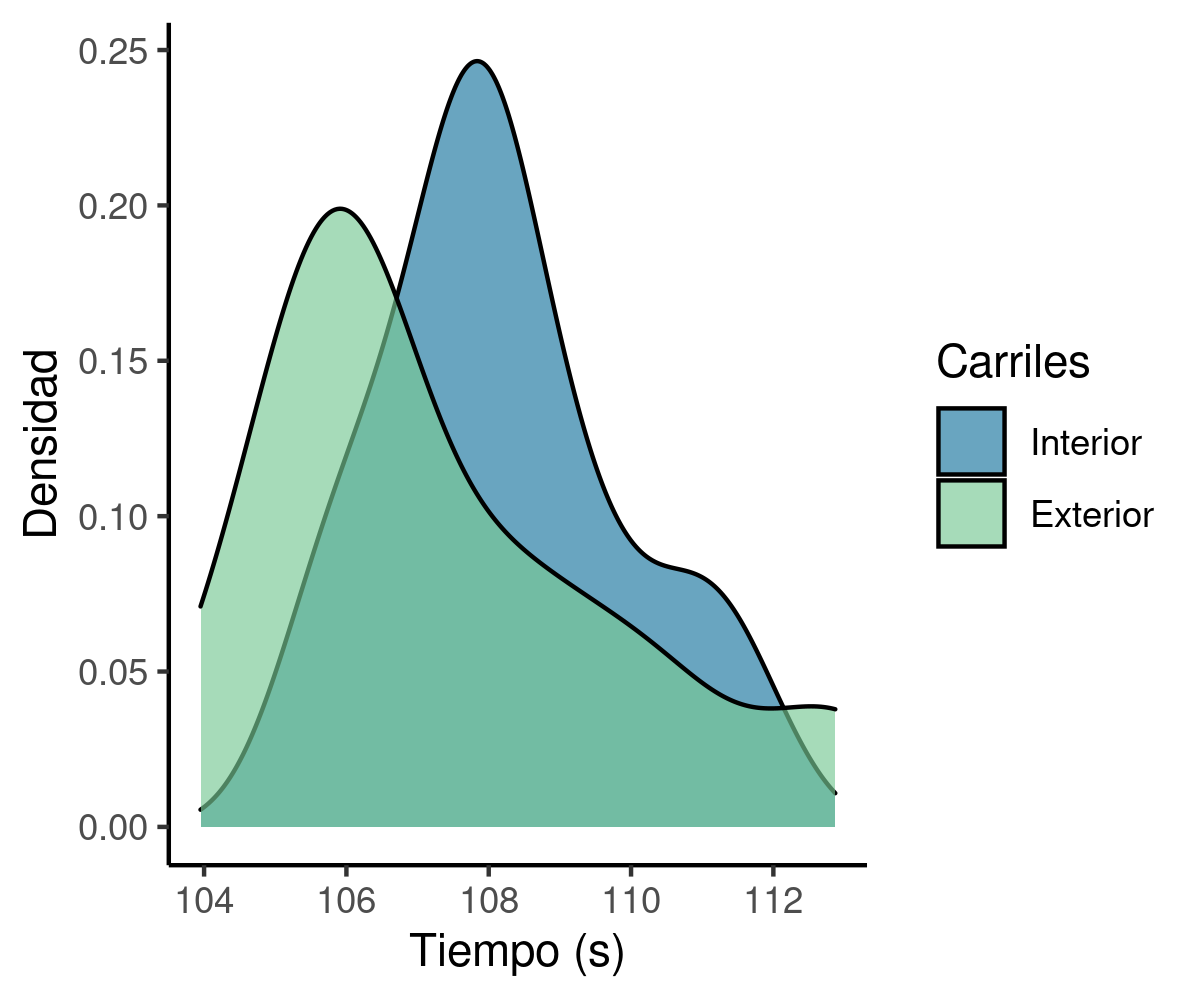
\includegraphics[width=8cm]{Graphics/problema07_histogram_2.png}
		\caption{Distribución de los datos del carril interior y exterior.}
		\label{fig:problema07_distribucion_datos}
	\end{subfigure}
	\caption{Representación gráfica de la distribucion de los datos.}
\end{figure}

En la tabla \ref{table:problema07} se observa que las varianzas muestrales son diferentes, por ende, al estar basadas en un estimador insesgado, entonces las varianzas de los datos son diferentes. Entonces el nonpooled variance (agregar cita) puede ser calculado como:

\begin{equation*}
	S_d^2 = \frac{S_x^2}{n} + \frac{S_y^2}{n}
\end{equation*}

El cual es un estimador insesgado para $Var(\bar{X}-\bar{Y})$, entonces, se puede calcular un valor t de la siguiente manera:

\begin{equation*}
	T_d = \frac{\bar{X}-\bar{Y}}{S_d}
\end{equation*}

El calculo de $T_d$ con los datos, da como resultado $1.2343$. El cual es un valor lejano a 0, por ende, la hipótesis es rechaza. Otra manera de comprobar esto es obteniendo el intervalo de confianza para las diferencias de tiempos de una misma carrera. La frecuencia de las diferencias de tiempos se muestra en la figura \ref{fig:problema07_histogram}.
\begin{figure}[H]
	\centering
	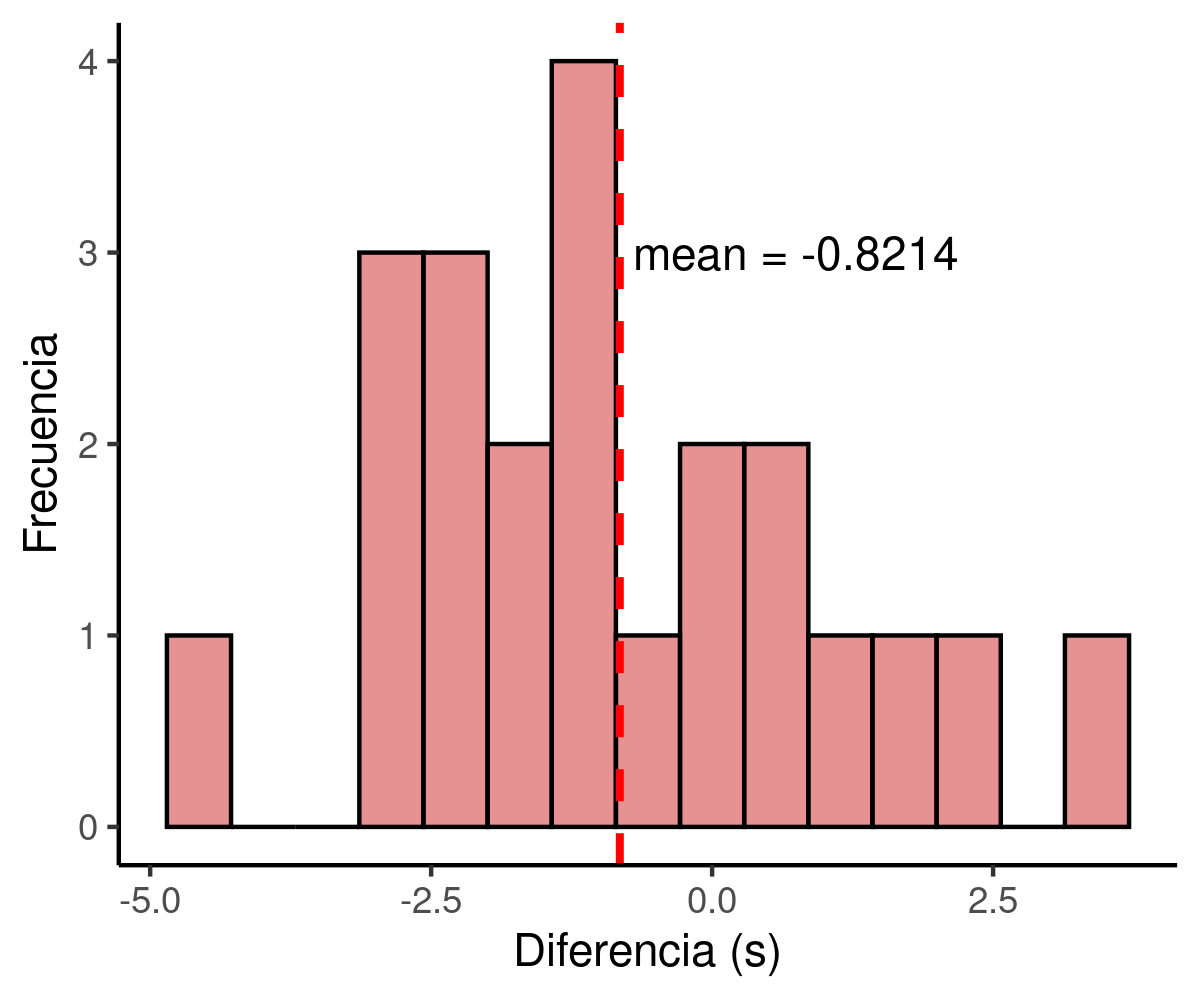
\includegraphics[width=10cm]{Graphics/problema07_histogram.png}
	\caption{Frecuencia de la diferencia entre los tiempos del carril exterior y carril interior.}
	\label{fig:problema07_histogram}
\end{figure}
